\section{The Cloud is Not Enough}
\label{sec:cloud-not-enough}

On the ``thing'' side, hardware platforms such as Arduino~\cite{arduino},
Raspberry Pi~\cite{rpi}, and BeagleBone Black~\cite{bbb} have allowed easy and
cheap prototyping for customized IoT applications.  Companies~\cite{ninja,
  smartthings, wink} in this space offer complete solutions including hardware
gateways, smartphone applications, web portals and cloud storage.

With this blizzard of activity, the current trend seems to be that all
peripherals, including sensors and actuators, communicate directly with the
cloud and interact with each other through web services~\cite{lee2014swarm}.  At
first glance, this seems to be a natural architecture for IoT applications.
However, several significant problems with this approach are revealed on closer
inspection, including issues with privacy, security, scalability, latency,
bandwidth and availability.  While these problems are not new to typical web
applications, they are exacerbated in the IoT space because of fundamental
differences between IoT and web services. The reasoning is as follows:

\begin{table}
  \centering
  \begin{tabular}{c c c}
    \toprule
    & Web/IT & Swarm/IoT \\
    \midrule
    Privacy \& Security & Open for access & Sensitive data \\
    Scalability & Power law & Billion devices \\
    Interaction Model & Human & Machine \\
    Latency & Variable & Bounded  \\
    Bandwidth & Downstream & Upstream   \\
    Availability (QoS) & No guarantee & Requirement  \\
    Durability Management & Cloud controls & Users control \\
    \bottomrule
  \end{tabular}
  \caption{Pitfalls with Today's Approach to directly using the cloud.}
\end{table}

\begin{enumerate}

\item \textbf{Privacy and Security.} Sensors implanted in our surrounding
  environment collect extremely sensitive information.  In a recent talk given
  by Wadlow~\cite{wadlow}, he described the IoT as ``hundreds of computers that
  are aware of me, can talk about me, and are out of my control.''  This is a
  strong call for intrinsic security and privacy.  This need is echoed in
  critical posts and talks---``Internet of Crappy
  Things''~\cite{alex2015internet}, ``The Internet of
  Fails''~\cite{stanislav2014the}, etc.  The FTC's Technical
  Report~\cite{ftc2015internet} also emphasizes security in the IoT spaces.  As
  a centralized resource out of users' control, the cloud presents an
  ever-present opportunity to violate privacy.  Today, privacy has become a
  luxury~\cite{angwin2014has}, a situation that will be exacerbated in the IoT.

\item \textbf{Scalability.} By 2020, Cisco estimates 50
  billion~\cite{evans2011internet} devices will be connected to the cloud, while
  Gartner estimates 26 billion~\cite{middleton2013forecast}. Scalability in the
  IoT spaces will be more challenging than web-scale or Internet-scale
  applications; the amount of data generated easily exceeds the reported
  trillion objects in Amazon S3~\cite{barr2013amazon}. The bisection bandwidth
  requirements for a centralized cloud solution are staggering, especially since
  most data acquired by IoT devices can or should be processed locally and
  discarded.

\item \textbf{Modeling: Peripheral devices are physical.}  Both sensors and
  actuators are physically present devices in our environment.  Although sensor
  data can be collected and replicated (similar to virtualizing
  sensors~\cite{yuriyama2010sensor}), the data is still generated from the edge
  of the network.  Moreover, actuators cannot be virtualized and oftentimes the
  actuations cannot be rolled back.  This is significantly different from the
  model of web services today.

\begin{figure}
  \centering
  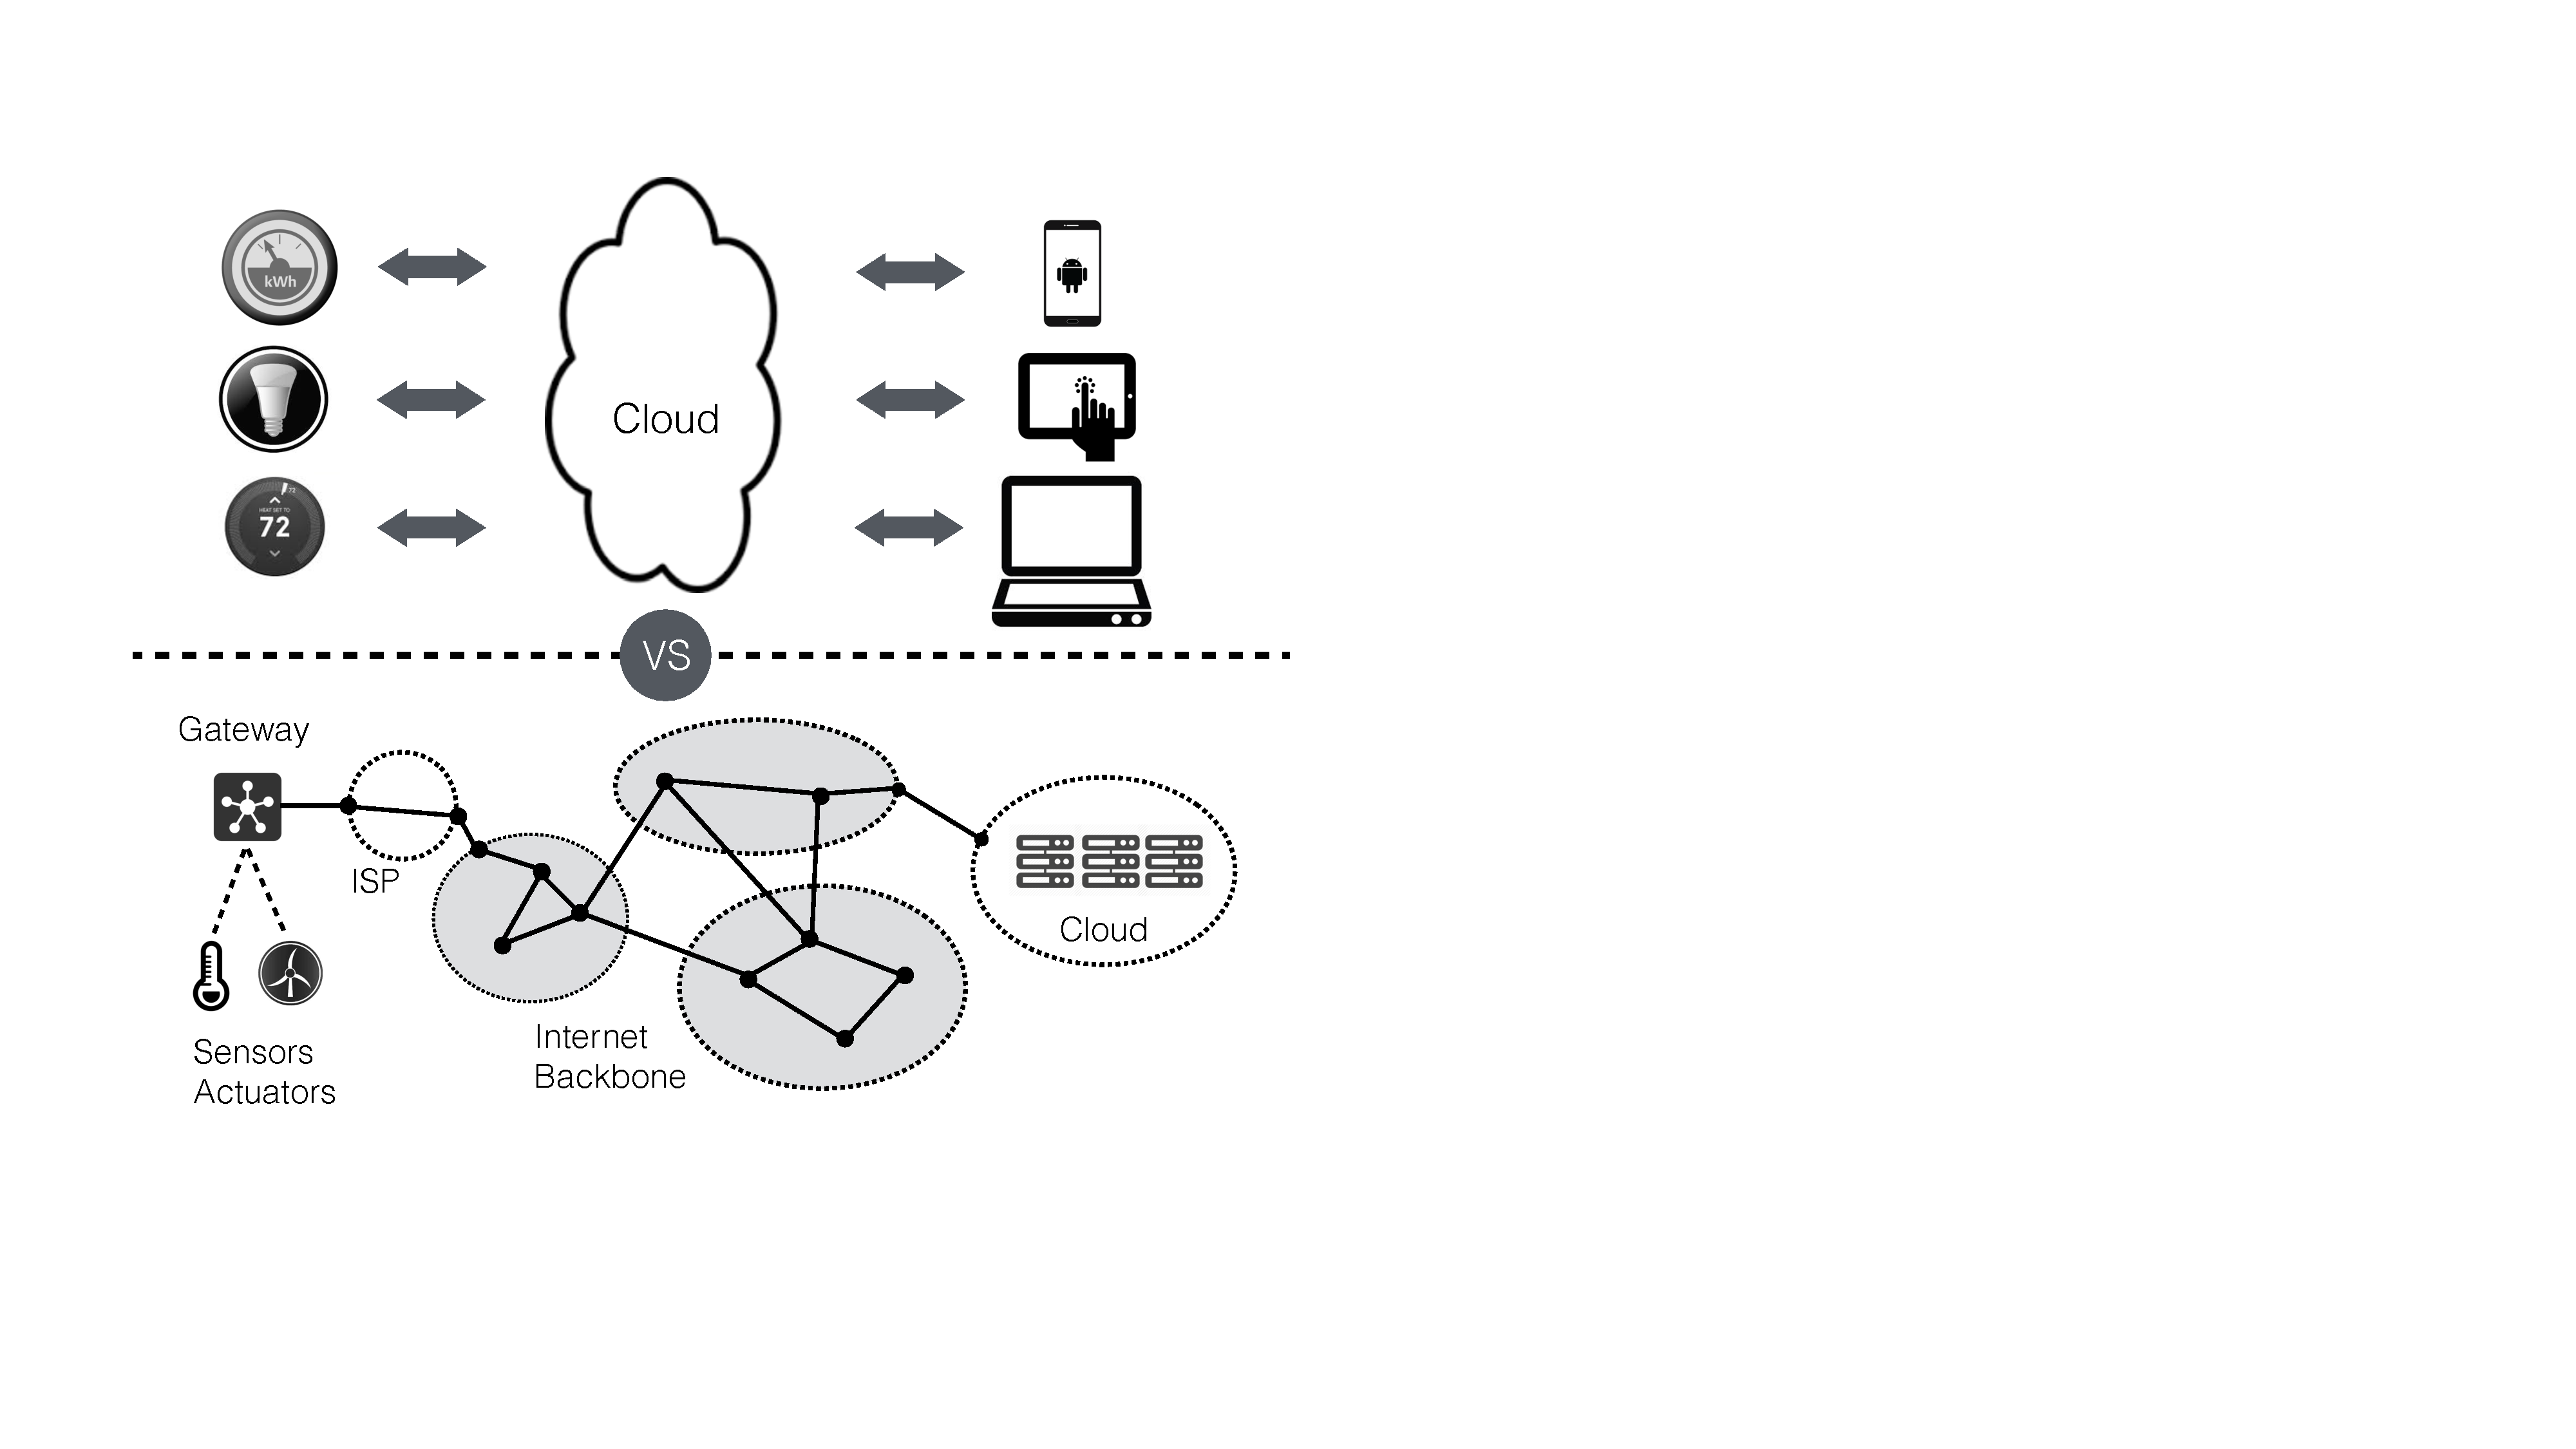
\includegraphics[width=0.6\columnwidth]{figures/cloud-view.pdf}
  \caption{Although applications usually view the cloud as the center of
    all connected devices (\textit{upper diagram}), in reality the cloud
    is usually on the edge of the Internet backbone, just like other
    devices (\textit{lower diagram}).}
  \label{fig:network}
\end{figure}

\item \textbf{Latency: The cloud model differs from reality.}  Application
  developers view the cloud as a component that interconnects the smart devices.
  However, from a network point of view, the cloud is on the edge of the network
  (see \autoref{fig:network}).  Even simple IoT applications, such as those that
  turn on a fan in response to a rise in local temperature, will experience
  unpredictable latencies from sensing, wireless transmission, gateway
  processing, Internet Service Provider (ISP), Internet, and cloud processing.

%% - sensor latency: 10-100 microseconds
%% - wireless latency: 676 µs (BLE, Overview and Evaluation of Bluetooth Low
%% Energy: An Emerging Low-Power Wireless Technology). Normally it's ~100 ms.
%% May need some data from http://iplane.cs.washington.edu/data/data.html

\item \textbf{Bandwidth: Upstream traffic dominates.}  Shipping data to the
  cloud incurs a significant amount of upstream traffic.  Typical broadband
  networks have more downstream bandwidth than upstream bandwidth.  IoT
  applications, however, generate data at the edges of the network, a pattern
  that will easily saturate the upstream link bandwidth---especially at scale.
  For example, a single Dropcam requires ``a high speed internet connection with
  at least 0.5 Mbps'' to use its service~\cite{dropcam}.  Even simple sensors,
  such as energy meters, can benefit from a higher sampling rate (the motivation
  of 1 kHz energy data with ground-truth from the Ubicomplab at the University
  of Washington~\cite{gupta2015household} and 15 kHz sampling of energy from MIT
  REDD Dataset~\cite{kolter2011redd}).

\item \textbf{Quality of Service (QoS) Guarantees.} Web users tolerate
  variable latency and occasional loss of web services.  In contrast, the
  temporary unavailability of sensors or actuators within IoT applications will
  directly impact the physical world.  While significant engineering effort has
  been put into improving the availability and latency profile of the cloud
  (allowing Service Level Agreements), such efforts are stymied by operator
  error, software bugs, DDoS attacks, and normal packet-to-packet variations
  from wide-area routing. Further, the Internet connection to people's homes is
  far from perfect.  Over 10\% of home networks in the developed world see
  connectivity interruptions of more than ten minutes more frequently than once
  every 10 days~\cite{grover2013peeking}; this situation is worse in developing
  countries.

\item \textbf{Durability Management.} Some sensor data is ephemeral: while other
  data should be durable against global disasters.  For ephemeral data, there is
  no effective way of verifying the data has been completely destroyed because
  the cloud is out of the user's control. For durable data, regardless of the
  promised guarantees~\cite{s3durability}, the reliability of cloud storage
  remains a major concern and there is active research in this
  direction~\cite{bessani2013depsky}.  Moreover, whatever durability is achieved
  by the cloud, it is typically done so without concern for application-specific
  privacy or export rules.  Note that control over durability is closely related
  to control in general: making sure that users retain control over their data
  rather than providers.

\end{enumerate}

%%% Local Variables:
%%% mode: latex
%%% TeX-master: "../background"
%%% End:
